\documentclass[final,hyperref={pdfpagelabels=false}]{beamer}
\usepackage{grffile}
\mode<presentation>{\usetheme{_bauer}}
\usepackage[english]{babel}
\usepackage[latin1]{inputenc}
\usepackage{amsmath, amsthm, amssymb, latexsym}
\usepackage{pifont} % for \ding symbols
\usepackage{multirow}
\usepackage{ragged2e} % for \justify
\let\olditem\item
\renewcommand\item{\justifying\olditem} % NOTE: This justify-alignes itemize-items, but heavily influences
% the rest of the document, s.t. the center-environment isn't working correctly anymore -> use \centering instead!

\usepackage{mdframed}
\newmdenv[%
  backgroundcolor=koalawhitegray4,
  linecolor=goodgreen,
  linewidth=3pt,
  topline=false,
  rightline=false,
  bottomline=false]{mdleftgreen}
\newmdenv[%
  backgroundcolor=koalawhitegray4,
  linecolor=badred,
  linewidth=3pt,
  topline=false,
  rightline=false,
  bottomline=false]{mdleftred}
  
%\usepackage{times}\usefonttheme{professionalfonts}  % obsolete
%\usefonttheme[onlymath]{serif}
%\boldmath % macht ALLE Gleichungen automatisch fett
\usepackage[orientation=portrait,size=a0,scale=1.4,debug]{beamerposter}
% change list indention level
% \setdefaultleftmargin{3em}{}{}{}{}{}



% Eigene Befehle und Einstellungen -------------------------
\newcommand{\grayHeader}[1]{\textcolor{koaladarkgray}{{\large #1} \vspace{2ex}}}
\newcommand{\bfBlue}[1]{\textcolor{koaladarkestblue}{\textbf{#1}}}
\newcommand{\bfDarkgray}[1]{\textcolor{koaladarkgray}{\textbf{#1}}}
\newcommand{\blue}[1]{\textcolor{koaladarkestblue}{#1}}
\newcommand{\badred}[1]{\textcolor{badred}{#1}}
\newcommand{\goodgreen}[1]{\textcolor{goodgreen}{#1}}
\newcommand{\darkgray}[1]{\textcolor{koaladarkgray}{#1}}
\newcommand{\lightgray}[1]{\textcolor{koalagray}{#1}}
\newcommand{\fndarkgray}[1]{\textcolor{koaladarkgray}{\footnotesize #1}}
\newcommand{\fnlightgray}[1]{\textcolor{koalagray}{\footnotesize #1}}
\newcommand{\colHeader}[1]{
  \vspace{-3ex}
  \begin{center}\centering
  \bfBlue{#1}
  \end{center}
  \vspace{-2ex}
  \textcolor{koalablue}{\hrule{}}
  \vspace{2ex}
}
% Numbers with circles around it for headers
\usepackage{tikz}
\newcommand*\circled[1]{\tikz[baseline=(char.base)]{
\node[shape=circle,draw,inner sep=2pt] (char) {#1};}}
% Make figures get numbers (Figure 1, ...)
\setbeamertemplate{caption}[numbered]
% Change style of figure caption label
\usepackage[font={footnotesize,it,color=black}]{caption}
\captionsetup[figure]{labelfont={color=black}}
\captionsetup[figure]{labelfont=bf}
% Highlight text parts with a color block with rounded corners
\usepackage{tcolorbox}
\newtcbox{\mybox}{nobeforeafter,colframe=chocolate4,colback=verylightgray,boxrule=2pt,arc=4pt,
  boxsep=0pt,left=6pt,right=6pt,top=6pt,bottom=6pt,tcbox raise base}
% Eigene Befehle Ende --------------------------------------



%\usepackage{snapshot} % will write a .dep file with all dependencies, allows for easy bundling

\usepackage{array,booktabs,tabularx}
\newcolumntype{Z}{>{\centering\arraybackslash}X} % centered tabularx columns
\newcommand{\pphantom}{\textcolor{ta3aluminium}} % phantom introduces a vertical space in p formatted table columns??!!
  
  \listfiles

%%%%%%%%%%%%%%%%%%%%%%%%%%%%%%%%%%%%%%%%%%%%%%%%%%%%%%%%%%%%%%%%%%%%%%%%%%%%%%%%%%%%%%
\graphicspath{{figures/}}

\title{\huge{KOALA: Estimating coalition probabilities}\\[0.5ex]\LARGE{in multi-party electoral systems}}
\author{Alexander Bauer$^{1}$, Andreas Bender$^{1}$, Andr\'e Klima$^{1}$, Helmut K\"{u}chenhoff$^{1}$}
\institute[LMU Munich]{\textit{$^{1}$ Statistical Consulting Unit StaBLab, Department of Statistics, LMU Munich,
Germany} \\[2ex] \texttt{Alexander.Bauer@stat.uni-muenchen.de}}
\date[July 18th, 2018]{July 18th, 2018}

%%%%%%%%%%%%%%%%%%%%%%%%%%%%%%%%%%%%%%%%%%%%%%%%%%%%%%%%%%%%%%%%%%%%%%%%%%%%%%%%%%%%%%
  \newlength{\columnheight}
\setlength{\columnheight}{105cm}


%%%%%%%%%%%%%%%%%%%%%%%%%%%%%%%%%%%%%%%%%%%%%%%%%%%%%%%%%%%%%%%%%%%%%%%%%%%%%%%%%%%%%%

% Begin page ----------------------------------------------
\begin{document}
\begin{frame}
\begin{columns}
\begin{column}{1\textwidth} % 1 Seite, die die ganze Seite einnimmt


% Motivation ---------------------------------------------
\begin{beamercolorbox}[center,wd=\textwidth]{postercolumn}
\begin{minipage}[T]{.95\textwidth}  % tweaks the width, makes a new \textwidth
\begin{block}{\footnotesize Motivation}
  \begin{center}\centering
  \grayHeader{Election poll-based reporting}
  \end{center}

  % Upper columns with general description -----
  \begin{columns}[t]

  \begin{column}{.475\textwidth}
  \colHeader{What's the status quo?}
  Typical election poll reporting: \\[1cm]
  \begin{tabular}{p{7.5cm}p{25cm}}
  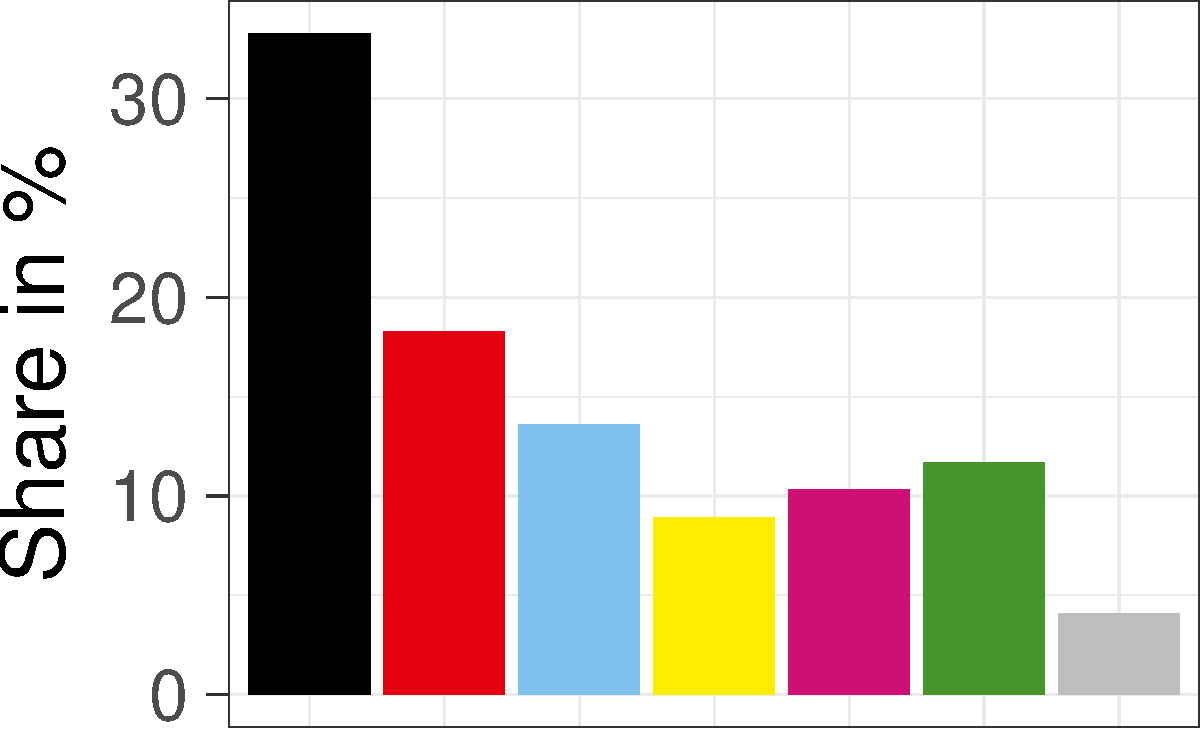
\includegraphics[height=4.75cm]{figures/motivation_survey}
  &
  \vspace{-4.5cm}
  \begin{itemize}
    \item is based on observed mean voter shares
    \item sets the focus on individual party achievements
    \item imparts sample uncertainty only insufficiently
  \end{itemize}
  \end{tabular}
  \\[2.5ex]
  % Example header
  {
  \setlength{\fboxrule}{3pt} % Border thickness
  \fcolorbox{koalawhitegray}{koalawhitegray2}{
  \begin{minipage}{0.9\textwidth}
  \vspace{2.5ex}
  \begin{center}\centering
  \bfBlue{Example} \\
  {\footnotesize \lightgray{Reporting on}} \darkgray{Union} {\footnotesize \lightgray{and}} \darkgray{FDP} {\footnotesize \lightgray{to jointly obtain a majority before the German federal election 2013}}
  \end{center}
  \vspace{2ex}
  \end{minipage}
  }
  }
  \end{column}

  % \hspace{-3.1ex}
  % \textcolor{LMUlightgray}{\vrule{}}
  % \hspace{3.1ex}
  
  \begin{column}{.475\textwidth}
  \colHeader{What do we propose?}
  Good reporting:
  \vspace{2.5ex}
  \begin{itemize}
    \item should impart findings in an easily graspable way
    \item should prevent potential misunderstandings
    \item should focus on the most relevant topics
  \end{itemize}
  \vspace{6.2ex}
  We aim at \textbf{shifting the focus} from \\[1.3ex]
  \begin{tabular}{clccl}
  \multirow{2}{*}[-0.95ex]{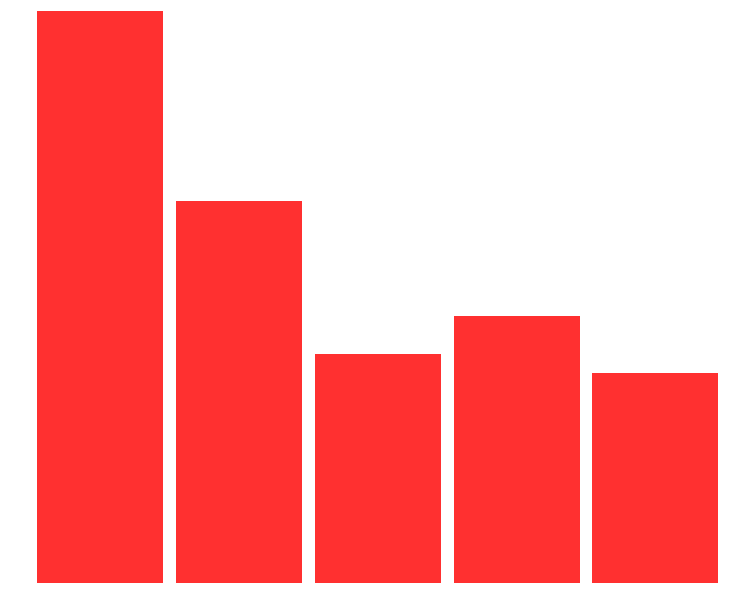
\includegraphics[height=3ex]{figures/motivation_pictoBar_col}} & 
  \darkgray{\footnotesize Incomprehensive} &
  \multirow{2}{*}{\ \ \darkgray{to} \ } &
  \multirow{2}{*}[-1ex]{
\includegraphics[height=3ex]{figures/motivation_pictoDens_col}} & 
  \darkgray{\footnotesize Uncertainty-based} \\
   & observed party shares & & & event probabilities \\
  \end{tabular}
  \end{column}

  \end{columns}
  
  % \noindent\hfil\textcolor{LMUlightgray}{\rule{0.93\textwidth}{.4pt}}\hfil
  % % \textcolor{LMUlightgray}{\hrule{}}
  % \vspace{3ex}
  
  % Lower columns with a specific example ----
  {
  \vspace{-4pt}
  \hspace{-24.34pt}
  \setlength{\fboxrule}{3pt} % Border thickness
  \fcolorbox{koalawhitegray}{koalawhitegray3}{
  \begin{minipage}{.96\textwidth}
  \vspace{3ex}
  \begin{columns}[t]

  \begin{column}{.29\textwidth}
  \darkgray{Last pre-election opinion poll:} \lightgray{\tiny Source: Forsa, 20.09.2013}
  \\[2.5ex]
  \begin{center}\centering
  % \scalebox{0.75} & {\footnotesize \lightgray{26\%}} & {\footnotesize \lightgray{10\%}} & \darkgray{5\%} & {\footnotesize \lightgray{9\%}} & {\footnotesize \lightgray{4\%}} & {\footnotesize \lightgray{6\%}} \\
  \bottomrule
  \end{tabular}
  % }
  \end{center}
  \vspace{1.5ex}
  \begin{center}\centering
  \darkgray{After redistribution} \lightgray{\footnotesize of party votes $<$5\% \\ (i.e. the minimum hurdle to pass into German parliament)} \\
  \darkgray{Union-FDP} \lightgray{\footnotesize jointly} \darkgray{obtain} \lightgray{\footnotesize exactly} \darkgray{50\%}.
  \end{center}
  \vspace{-3ex}
  \textcolor{koalablue}{$$ \underbrace{\resizebox{\hsize}{!}{ }}_{ } $$}
  \ \\ \vspace{-2ex}
  \begin{mdleftred}
  \begin{minipage}{\textwidth}
  \lightgray{\footnotesize Media headline:}
  \\
  \begin{center}\centering
  \vspace{-2ex}
  \darkgray{\textit{``Union-FDP loses its majority''}}
  \vspace{-.2ex}
  \end{center}
  \lightgray{\tiny Source: FAZ.net (2017). Umfrage zur Bundestagswahl: Schwarz-Gelb verliert \\[-2ex]
  die Mehrheit.http://archive.is/SuXVt. Accessed 26 April 2018.}
  \end{minipage}
  \end{mdleftred}
  \end{column}

  \begin{column}{.025\textwidth}
  \vspace{11ex}
  \huge{\blue{\ding{223}}}
  \end{column}

  \begin{column}{.26\textwidth}
  Flaws of this type of reporting:
  \vspace{1.5ex}
  \begin{itemize}
    \item \darkgray{Misleading conclusions are drawn} \\[0.2cm] \fnlightgray{A mean share of 50\% only means that it's} \fndarkgray{slightly more probable} \fnlightgray{that a majority is missed}
    \item \darkgray{Sample uncertainty is ignored} \\[0.2cm] \fnlightgray{E.g., with a mean voter share of 5\%, FDP will only enter the parliament with $\sim$50\%}
    \item \darkgray{Redistribution of votes is ignored} \\[0.2cm] \fnlightgray{FAZ.net bases the conclusion on the observed voter share and not on the redistributed 50\% share}
  \end{itemize}
  \end{column}

  \begin{column}{.025\textwidth}
  \vspace{11ex}
  \huge{\blue{\ding{223}}}
  \end{column}

  \begin{column}{.29\textwidth}
  Foundations of KOALA-based reporting:
  \vspace{1.5ex}
  \begin{itemize}
    \item \darkgray{Use event \textbf{probabilities}} \fnlightgray{instead of voter shares} \\[0.2cm] \fnlightgray{Probabilities comprise sample uncertainty in a natural way and are less at risk to be misinterpreted}
    \item \darkgray{Use \textbf{event} probabilities} \fnlightgray{instead of voter shares} \\[0.2cm] \fnlightgray{Focusing on the main events allows the reader to easily grasp the big picture}
  \end{itemize}
  \vspace{-1.7ex}
  \textcolor{koalablue}{$$ \underbrace{\resizebox{\hsize}{!}{ }}_{ } $$}
  \ \\ \vspace{-2ex}
  
  \begin{mdleftgreen}
  \begin{minipage}{\textwidth}
  \lightgray{\footnotesize KOALA headline:}
  \begin{center}\centering
  \darkgray{\textit{
  ``Union-FDP gains seat majority with 26\%, \ \ \\[0.1cm] \ \ FDP passes into parliament with 51\%$^*$''
  }}
  \end{center}
  \vspace{-0.7ex}
  \lightgray{\tiny ${}^*$ If the election was held today}
  \end{minipage}
  % }
  \end{mdleftgreen}
  \end{column}
  \end{columns}
  \end{minipage}
  }
  }

  \vspace{1ex}
\end{block}
\end{minipage}
\end{beamercolorbox}



% Begin main part -----------------------------------
\vspace{2ex}
\begin{columns}[T]

% empty space on left
\begin{column}{.016\textwidth}
\end{column}

\begin{column}{.484\textwidth}
\begin{beamercolorbox}[center,wd=\textwidth]{postercolumn}
\begin{minipage}[T]{.95\textwidth}  % tweaks the width, makes a new \textwidth
% \parbox[t][\columnheight]{\textwidth}{ % must be some better way to set the the height, width and textwidth simultaneously
% Since all columns are the same length, it is all nice and tidy.  You have to get the height empirically


% Methodology ---------------------------------------
\begin{block}{\footnotesize \circled{1} Event probability estimation}
We use a \bfBlue{Multinomial-Dirichlet model}
%with uninformative prior
for the true party shares $\theta_j$ {\footnotesize (Gelman et al., 2013)}:
$$
(\theta_1,\ldots,\theta_k)^T \sim Dirichlet(\alpha_1,\ldots,\alpha_k), \ \ \text{with} \ \ \alpha_1 = \ldots = \alpha_k = \frac{1}{2}
$$
% $$
% \begin{aligned}
% \boldmath{\theta} &= (\theta_1,\ldots,\theta_k)^\T \sim Dirichlet(\alpha_1,\ldots,\alpha_k), \\
% \text{with} &\ \ \ \ \ \ \ \ \ \ \ \ \ \ \ \alpha_1 = \ldots = \alpha_k = \frac{1}{2}
% \end{aligned}
% $$
Given one survey, the posterior also is a Dirichlet distribution
with $\alpha_j = x_j + \frac{1}{2}$ for each party $j$ and its observed
vote counts $x_j$.
\\[0.5cm]
Using \bfBlue{Monte Carlo simulations} of election outcomes, we obtain obtain
specific event probabilities by taking their relative frequency of
occurence.
% As vote shares are usually rounded before publication,
% we adjust the available data by adding random noise to $x_j$ before
% calculating the Bayesian posterior.
% we add uniformly distributed random noise $r_\gamma \sim U[-\gamma,\gamma]$ to the shares (e.g., $\gamma = 0.5\%$) and rescale the sum to $100\%$.

\vspace{1ex}
\textcolor{LMUlightgray}{\hrule{}}
\vspace{3ex}

% In the presence of multiple published opinion polls, pooling is used to summarize the observed results in order to reduce sample uncertainty. To assure a reliable pooling regarding the current public opinion, we only use polls published within the past 14 days and only use the most recent survey published by each polling agency.
\bfBlue{Pooling} is used to summarize multiple polls to reduce sample uncertainty:
\begin{itemize}\vspace{0.4cm}
  \item We pool the most recent survey per polling agency within the past 14 days
  \item The summed number of votes per party are also multinomially distributed
  \item \textbf{\badred{But:}} Polls from different polling agencies are correlated
\vspace{0.4cm}\end{itemize}
% To reliably estimate the current public opinion, we use polls published within the past 14 days, only using the most recent survey per polling agency.
% To assure a reliable pooling regarding the current public opinion, we only use polls published within the past 14 days and only use the most recent survey published by each polling agency.
% As vote counts $X_{ij}$ of party $j$ in poll $i$ are multinomially distributed, so are the summed number of votes $\sum_i X_{ij}$ when pooling multiple independent polls.
% Looking at a single poll $i$, the observed number of votes $X_j$ for each of $k$ parties follow a multinomial distribution with sample size $n_i$ and underlying, unknown party shares $\theta_j$ in the population:
% $$
% X_1,\ldots, X_k \sim Multinomial(n_i,\theta_1,\ldots,\theta_k).
% $$
% Based on the multinomial distribution of the vote counts $X_{ij}$ of party $j$ in poll $i$, pooling over multiple polls as independent random samples leads to another multinomial distribution for the summed number of votes $\sum_i X_{ij}$.
% Based on the multinomial distribution of the vote counts $X_{ij}$ of party $j$ in poll $i$ with underlying true party share $\theta_j$, pooling over multiple polls representing independent random samples would lead to a multinomial distribution for the summed number of votes $\sum_i X_{ij}$:
% $$
% \sum\limits_i X_{i1},\ldots, \sum\limits_i X_{ik} \sim Multinomial(\sum\limits_i n_i,\theta_1,\ldots,\theta_k).
% $$
% However, polls from different polling agencies are correlated.
%Further analyses, however, show that polls from different
%polling agencies are correlated.
%and the independency assumption does not hold.
\textbf{\goodgreen{Hence:}} We adjust the
%resulting multinomial
distribution by using an \bfBlue{effective sample size} {\footnotesize (Hanley et al., 2003)}:
Party-specific correlations were estimated based on
20 surveys of polling agencies Emnid and Forsa, using
$$
Cov(X_{Aj}, X_{Bj}) = \frac{1}{2} \cdot \left(Var(X_{Aj}) + Var(X_{Bj}) - Var(X_{Aj} - X_{Bj}) \right),
$$
with
\begin{itemize}
  \item $Var(X_{Aj})$, $Var(X_{Bj})$ the theoretical variances of binomial distributions,
  \item $Var(X_{Aj} - X_{Bj})$ estimated from the party share differences.
\end{itemize}
For simplicity, we set the correlation to a fixed value of $0.5$.
% For simplicity, we do not recalculate the correlation for each simulation, but rather set the correlation to $0.5$, based on the initial calculation discussed above.
The effective sample size $n_{\text{eff}}$ is then defined as the ratio between
the estimated variance for the pooled sample and the theoretical variance for a
sample of size one:
$$
n_{\text{eff}} = \frac{Var(\text{pooled})}{Var(\text{sample of size one})}.
$$
% For convenience, this calculation is based on the party with most votes,
% as the specific party choice only marginally affects the results.

% Quantification of pairwise correlation is done based on the variance of the
% difference between two polls. The following equation holds for two independent
% random sample polls $A$ and $B$:
%
% $$
% \begin{aligned}
% %Var(X_A - X_B) &= Var(X_A) + Var(X_B) - 2 \cdot Cov(X_A, X_B) \\
% Cov(X_{Aj}, X_{Bj}) &= \frac{1}{2} \cdot \left(Var(X_{Aj}) + Var(X_{Bj}) - Var(X_{Aj} - X_{Bj}) \right).
% \end{aligned}
% $$
%
% We take $Var(X_{Aj})$ and $Var(X_{Bj})$ as the theoretical variances of the binomially distributed, observed voter numbers and estimate $Var(X_{Aj} - X_{Bj})$ based on the observed differences between the party shares. Having done so, one can estimate the covariance $Cov(X_{Aj}, X_{Bj})$ and accordingly also the correlation. As the binomial distribution is directly proportional to the sample size, the effective sample size $n_{\text{eff}}$ can be defined as the ratio between the estimated variance for the pooled sample and the theoretical variance of a sample of size one:
% $$
% n_{\text{eff}} = \frac{Var(\text{pooled})}{Var(\text{sample of size 1})},
% $$
% with, in the case of two surveys,
% $$
% Var(\text{pooled}) = Var(X_A + X_B) = Var(X_A) + Var(X_B) + 2 Cov(X_A,X_B)
% $$
% and $Var(\text{sample of size 1})$ the theoretical variance of the pooled share.
%
% Looking at the party-specific correlations between 20 surveys conducted by the two most regular German polling agencies, Emnid and Forsa, we on average end up with a medium high correlation, using mean party shares and sample sizes per institute for the theoretical variances. Other institute comparisons were not performed as too few surveys were conducted over comparable time frames. For simplicity, we set the correlation used in our methodology to $0.5$. For calculating $n_{\text{eff}}$ we base the calculation on the result of the biggest party, as the specific party choice only marginally affects $n_{\text{eff}}$.
\end{block}



% Begin second column of main part -----------------
\end{minipage}
\end{beamercolorbox}
\end{column}

\begin{column}{.484\textwidth}
\begin{beamercolorbox}[center,wd=\textwidth]{postercolumn}
\begin{minipage}[T]{.95\textwidth}  % tweaks the width, makes a new \textwidth


% Visualization ------------------------------------
\begin{block}{\footnotesize \circled{2} Visualization}
To visualize the development of such probabilities together with the underlying uncertainty for a specific coalition we use \bfBlue{ridgeline plots} (Wilke, 2017) for the simulated seat distributions:
\begin{center}\centering
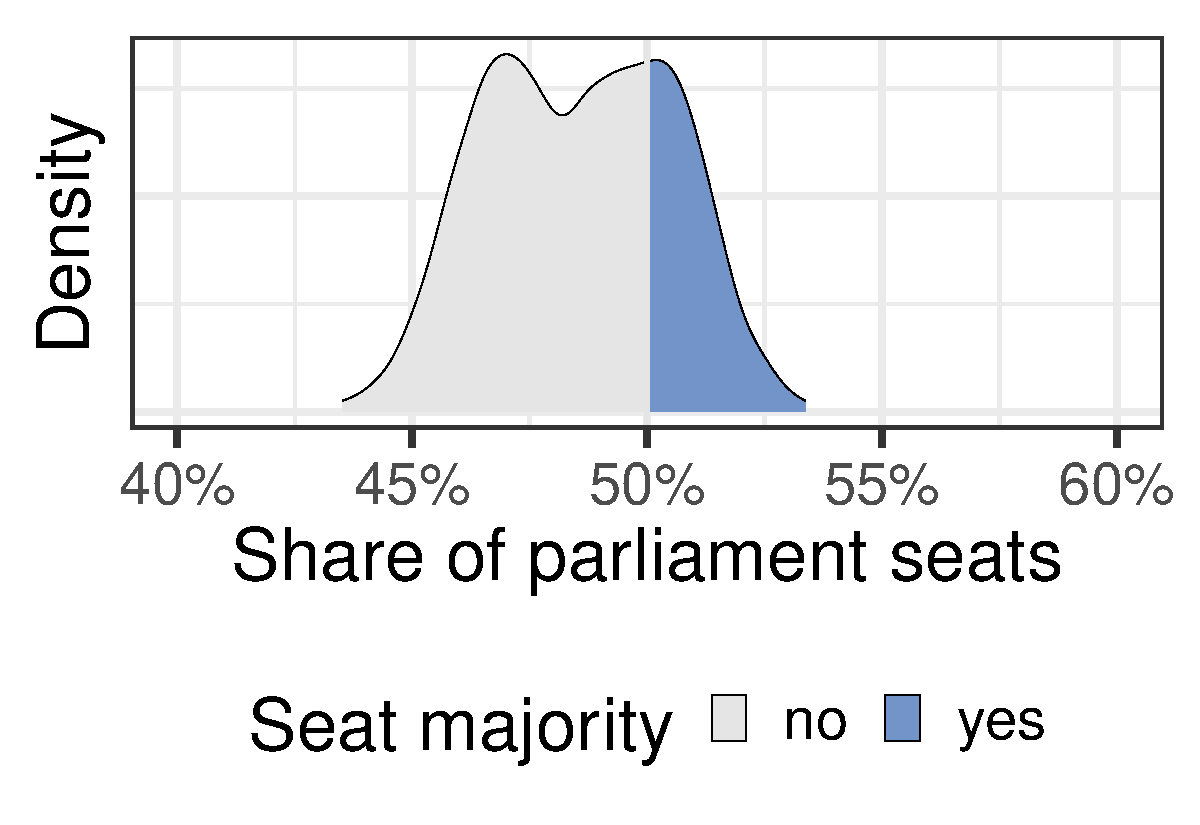
\includegraphics[height=12ex]{figures/vis_seatDist}
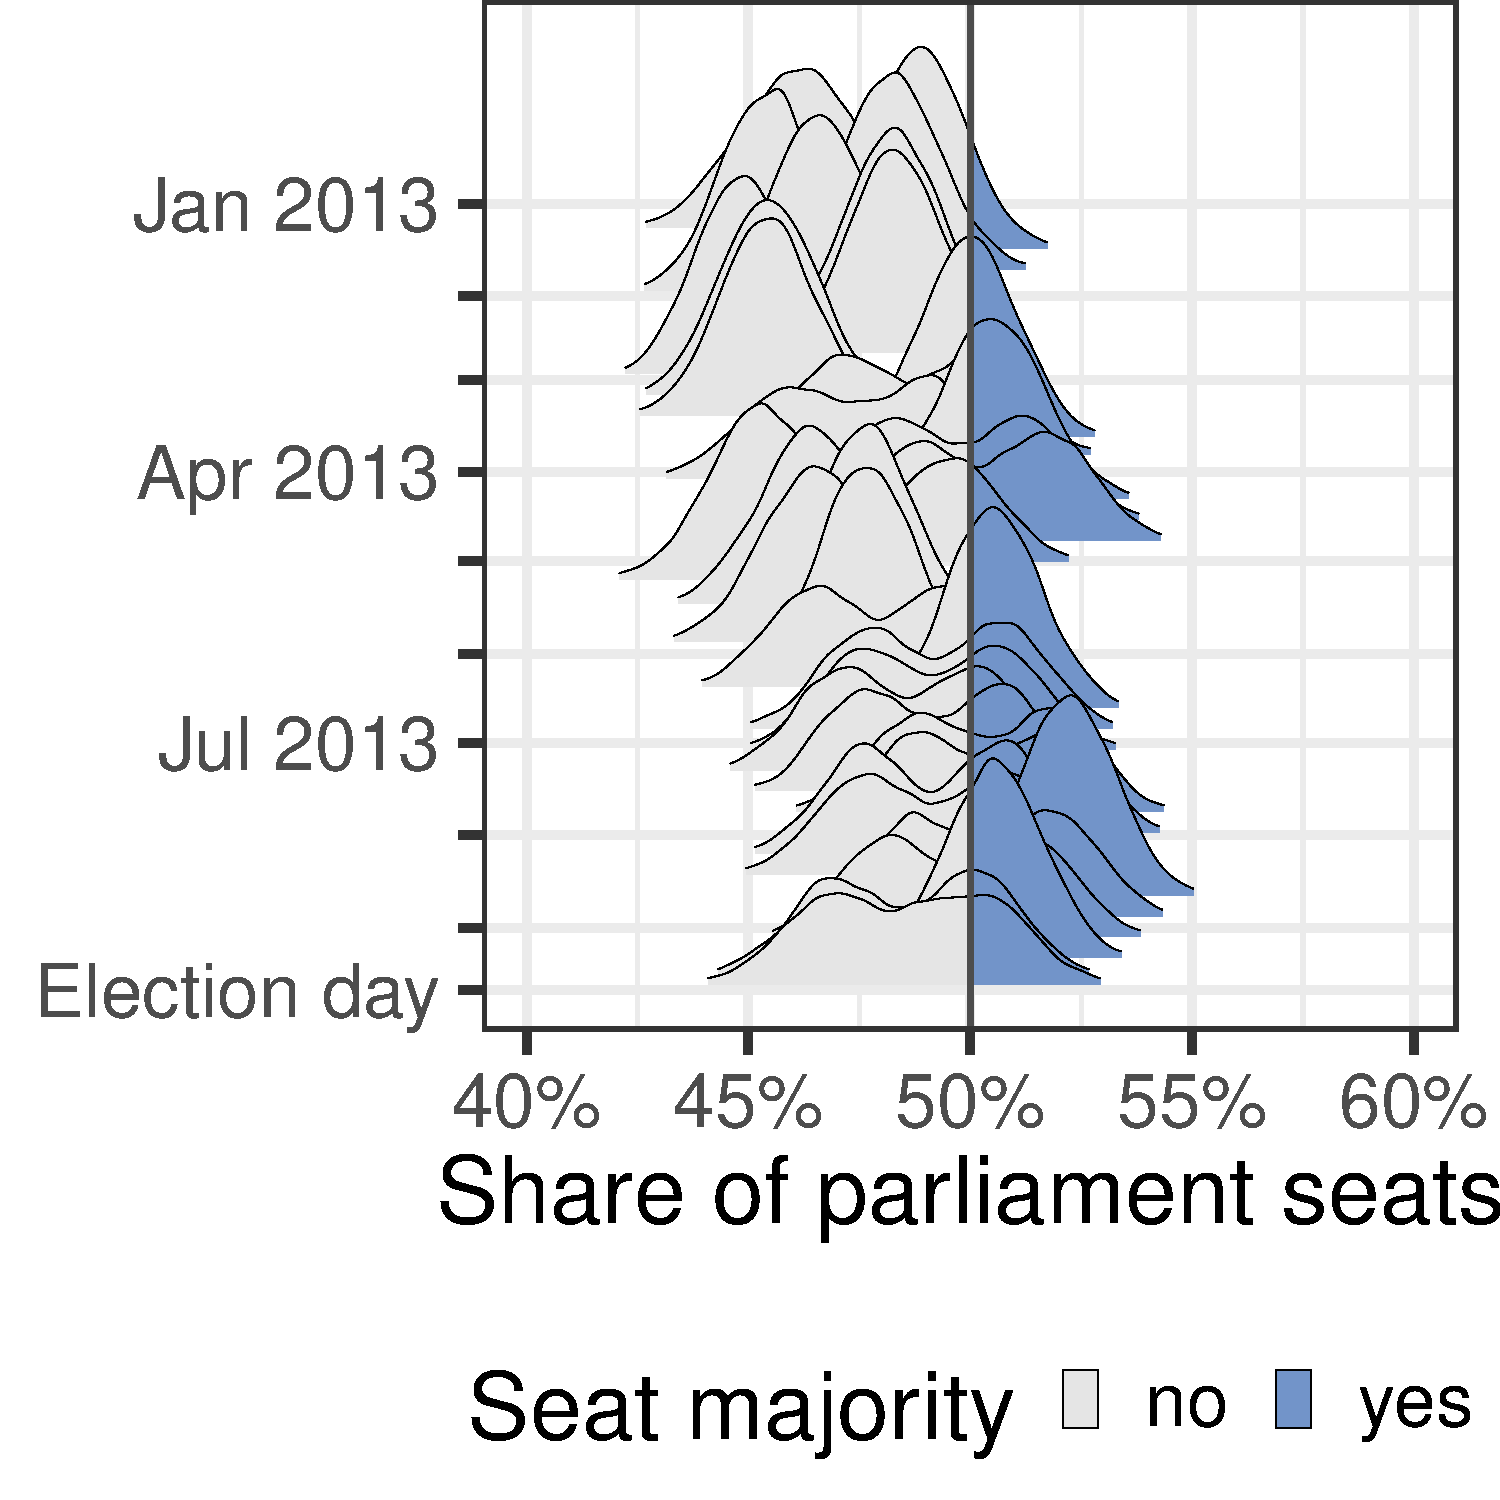
\includegraphics[height=20ex]{figures/vis_seatDist_time}
\end{center}
Looking at the probabilities based on the last opinion poll before the German election 2013, the posterior distribution is bimodal, based on the distinction whether FDP and/or AfD pass the 5\% hurdle. The resulting probability for a Union-FDP majority is 27.2\%, based on $10,000$ simulations.
\end{block}


% Implementation -----------------------------------
\begin{block}{\footnotesize \circled{3} Implementation and results communication}
\begin{center}\centering

\includegraphics[height=5ex]{figures/Koala_Logo_ohneSchrift}
\\[2ex]
Results for selected elections are presented on
\bfBlue{\texttt{\href{http://koala.stat.uni-muenchen.de}{koala.stat.uni-muenchen.de}}}
\end{center}
\vspace{2ex}
The implementation is based on several points:
\begin{itemize}
  \item Our approach is implemented in the R package \bfBlue{\texttt{coalitions}} 
  \item The website is shiny-based
  \item The website update approach is automated
  \item Automatic tweets are sent in the case of new results
  \item For sharing our results we automatically export them to Google Sheets
\end{itemize}

% Footer with software icons
\vspace{1ex}
\textcolor{LMUlightgray}{\hrule{}}
\vspace{1ex}
\begin{columns}[t]
  \begin{column}{.15\textwidth}
  \begin{center}\centering
  
\includegraphics[height=5ex]{figures/implementation_r}
  \end{center}
  \end{column}

  \hspace{-1.5ex}
  \textcolor{LMUlightgray}{\vrule{}}
  \hspace{1.5ex}

  \begin{column}{.15\textwidth}
  \begin{center}\centering
  \vspace{1ex}
  
\includegraphics[height=3ex]{figures/implementation_shiny}
  \end{center}
  \end{column}

  \hspace{-1.5ex}
  \textcolor{LMUlightgray}{\vrule{}}
  \hspace{1.5ex}

  \begin{column}{.15\textwidth}
  \begin{center}\centering
  
\includegraphics[height=5ex]{figures/hexSticker_icon}
  \end{center}
  \end{column}

  \hspace{-1.5ex}
  \textcolor{LMUlightgray}{\vrule{}}
  \hspace{1.5ex}

  \begin{column}{.15\textwidth}
  \begin{center}\centering
  
\includegraphics[height=5ex]{figures/implementation_sheets}
  \end{center}
  \end{column}

  \hspace{-1.5ex}
  \textcolor{LMUlightgray}{\vrule{}}
  \hspace{1.5ex}

  \begin{column}{.15\textwidth}
  \begin{center}\centering
  
\includegraphics[height=5ex]{figures/implementation_twitter}
  \end{center}
  \end{column}
\end{columns}
\end{block}


% End main part ------------------------------------
\end{minipage}
\end{beamercolorbox}
\end{column}

% empty space on right
\begin{column}{.016\textwidth}
\end{column}

\end{columns}


% Literature ---------------------------------------
\vspace{2ex}
\begin{beamercolorbox}[center,wd=\textwidth]{postercolumn}
\begin{minipage}[T]{.95\textwidth}  % tweaks the width, makes a new \textwidth
\begin{block}{\footnotesize References}
{\footnotesize
Bender, A. and Bauer, A. (2018). coalitions: Coalition probabilities in multi-party democracies.
\textit{Journal of Open Source Software}, \textbf{3(23)}, 606,
\href{https://doi.org/10.21105/joss.00606}{\texttt{https://doi.org/10.21105/joss.00606}}. \\
Unser AStA-Paper no ois Technical Report? \\
Gelman, A. et al. (2013). \textit{Bayesian Data Analysis, 3rd edition}. Boca Raton, FL: CRC press. \\
Hanley, J. A. et al. (2003). Statistical analysis of correlated data using gen-
eralized estimating equations: an orientation. \textit{American journal of epidemiology},
\textbf{157(4)}, 364--375. \\
Wilke C.O. (2017). \textit{ggridges: Ridgeline Plots in 'ggplot2'}. R package version
0.4.1. URL \href{https://CRAN.R-project.org/package=ggridges}{https://CRAN.R-project.org/package=ggridges}
}
\end{block}
\end{minipage}
\end{beamercolorbox}

% End page -----------------------------------------
\end{column} % 1 Spalte, die die ganze Seite einnimmt
\end{columns}
\end{frame}
\end{document}
  
  
  %%%%%%%%%%%%%%%%%%%%%%%%%%%%%%%%%%%%%%%%%%%%%%%%%%%%%%%%%%%%%%%%%%%%%%%%%%%%%%%%%%%%%%%%%%%%%%%%%%%%
    %%% Local Variables: 
    %%% mode: latex
  %%% TeX-PDF-mode: t
  %%% End:
    